\documentclass[13pt]{beamer}
\usepackage{graphicx}
\usepackage[utf8]{inputenc}
\usepackage[skip=2pt,font=scriptsize]{caption}

% Captions
\captionsetup{labelformat=empty,labelsep=none}

% References
\usepackage{url}
\bibliographystyle{acm}
\setbeamertemplate{bibliography item}[triangle]

% Formatting
\usetheme{Singapore}
\usecolortheme{whale}

% Title Page
\title{Binomial Heap}
\author{Introduction and Exercises}
\institute{Devin Delfino}
\date{3/05/2014}

\begin{document}
% TITLE ------------------------------------------------
\frame{\titlepage}

% BINOMIAL TREES ------------------------------------------------
\begin{frame}
\frametitle{Binomial Trees}
	\begin{itemize}
		\item A \alert{Binomial Tree} is a specific type of tree that includes the following specifications:
          \begin{enumerate}
            \item The \alert{order} or \alert{rank} of the binomial tree is the number of children of the root node.
            \item A Binomial Tree of order $0$ is a single node.
            \item A Binomial Tree of order $k$ has $k$ child nodes, all of which are the roots of binomial trees of orders $k - 1$, $k - 2$, ..., 2, 1, 0 from left to right.
          \end{enumerate}
	\end{itemize}
\end{frame}

% Exercise #1 ------------------------------------------------
\begin{frame}
\frametitle{Excercise: Binomial Trees}
  \begin{itemize}
    \item Determine the order of the following binomial trees (note how if the tree has order \textit{k}, the orders of the child nodes decrease from left to right from $k-1$ to $0$).
  \end{itemize}

  \begin{columns}[T] % the "c" option specifies center vertical alignment
    \begin{column}[T]{3.3cm} % alternative top-align that's better for graphics
      \begin{figure}
        \caption{Figure 1}
        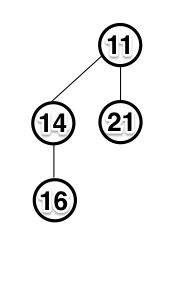
\includegraphics[height=4cm]{order2.png}
      \end{figure}
      \centering
    \end{column}
    \begin{column}[T]{3.3cm} % alternative top-align that's better for graphics
      \begin{figure}
        \caption{Figure 2}
        
\includegraphics[height=4cm]{order0.png}
      \end{figure}
    \end{column}
    \begin{column}[T]{3.3cm} % alternative top-align that's better for graphics
      \begin{figure}
        \caption{Figure 3}
        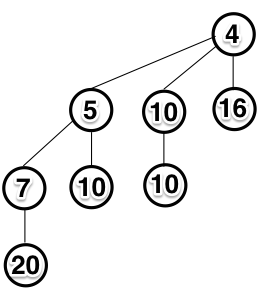
\includegraphics[height=4cm]{order3.png}
      \end{figure}
      \centering
    \end{column}
    \begin{column}[T]{3.3cm} % alternative top-align that's better for graphics
      \begin{figure}
        \caption{Figure 4}
        
\includegraphics[height=4cm]{order1.png}
      \end{figure}
    \end{column}
  \end{columns}

\end{frame}

% BINOMIAL HEAP ------------------------------------------------
\begin{frame}
\frametitle{Binomial Heaps}
  \begin{itemize}
    \item A \alert{Binomial Heap} is a collection of binomial trees that satisfy the following two binomial heap properties:
      \begin{enumerate}
        \item The key of any node is greater than or equal to the key of its parent (minimum-heap property).
        \item There cannot be two binomial trees of the same order.
      \end{enumerate}
    \item The first property (minimum-heap) ensures that the root is the smallest key in each binomial tree. Similarly, the smallest key of the entire heap is one of the roots.
    \item The second property ensures that the if a binomial heap has \textit{n} nodes, then it will have at most $\lfloor \textit{log n} \rfloor + 1$ binomial trees.
    \item Binomial heaps are used to implement priority queues.
  \end{itemize}
\end{frame}

% Exercise #2 ------------------------------------------------
\begin{frame}
\frametitle{Excercise: Binomial Heap Property \#1}
  \begin{itemize}
    \item Determine if the following binomial trees satisfy the minimum-heap property.
  \end{itemize}

  \begin{columns}[T] % the "c" option specifies center vertical alignment
    \begin{column}[T]{6.5cm} % alternative top-align that's better for graphics
      \begin{figure}
        \caption{Figure 1}
        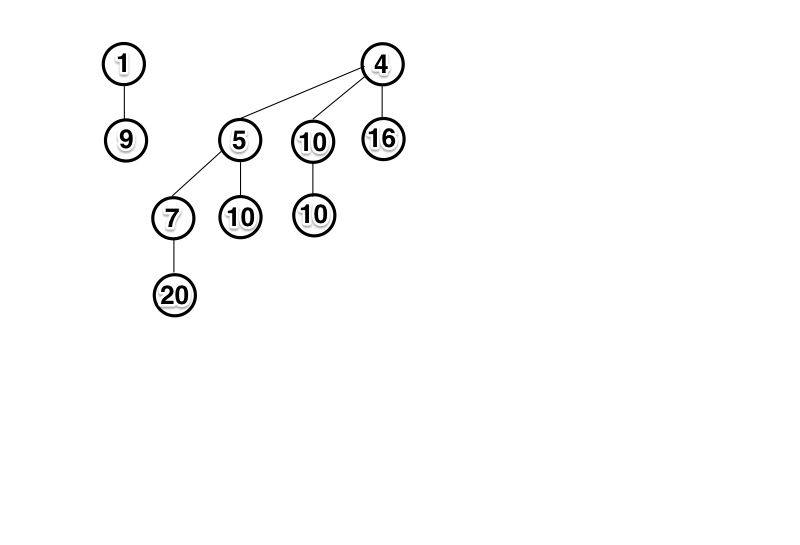
\includegraphics[height=7cm]{minheap1.png}
      \end{figure}
      \centering
    \end{column}
    \begin{column}[T]{6.5cm} % alternative top-align that's better for graphics
      \begin{figure}
        \caption{Figure 2}
        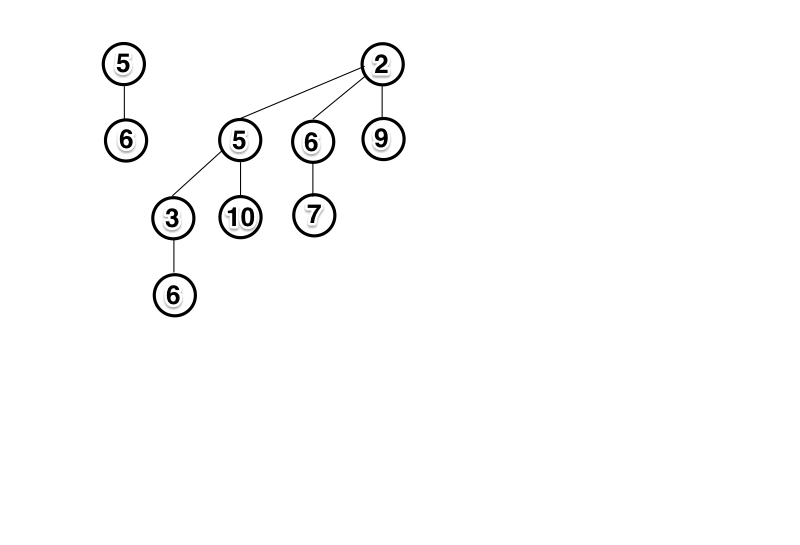
\includegraphics[height=7cm]{minheap2.png}
      \end{figure}
    \end{column}
  \end{columns}
\end{frame}

% Exercise #3 ------------------------------------------------
\begin{frame}
\frametitle{Excercise: Binomial Heap Property \#2}
  \begin{itemize}
    \item Determine if the following structures are valid Binomial Heaps.
  \end{itemize}

  \begin{columns}[T] % the "c" option specifies center vertical alignment
    \begin{column}[T]{4.3cm} % alternative top-align that's better for graphics
      \begin{figure}
        \caption{Figure 1}
        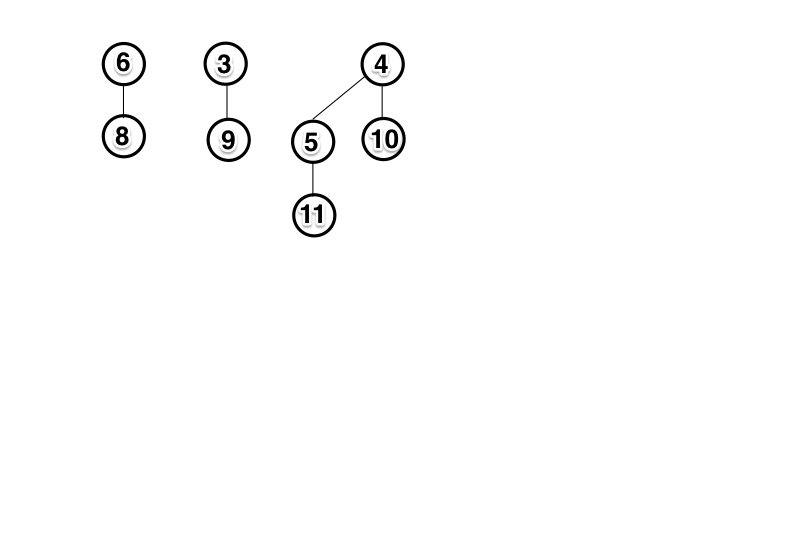
\includegraphics[height=5cm]{struct4.png}
      \end{figure}
      \centering
    \end{column}
    \begin{column}[T]{4.3cm} % alternative top-align that's better for graphics
      \begin{figure}
        \caption{Figure 2}
        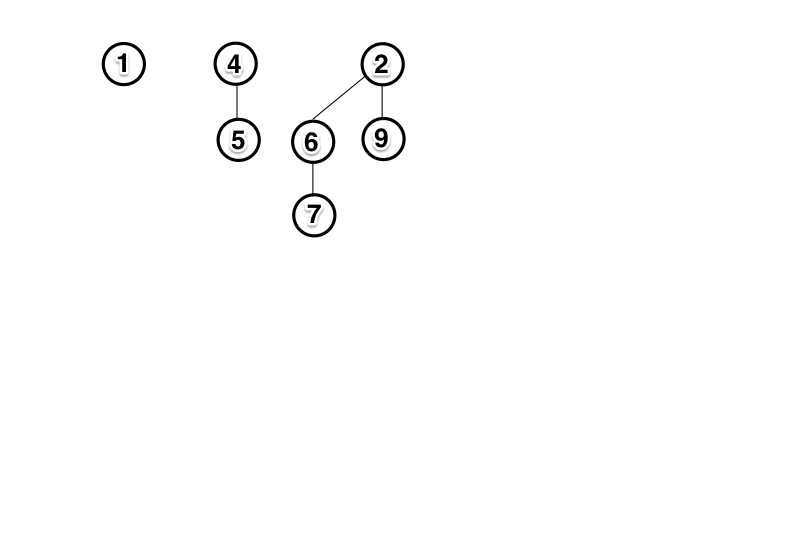
\includegraphics[height=5cm]{struct2.png}
      \end{figure}
    \end{column}
    \begin{column}[T]{4.3cm} % alternative top-align that's better for graphics
      \begin{figure}
        \caption{Figure 3}
        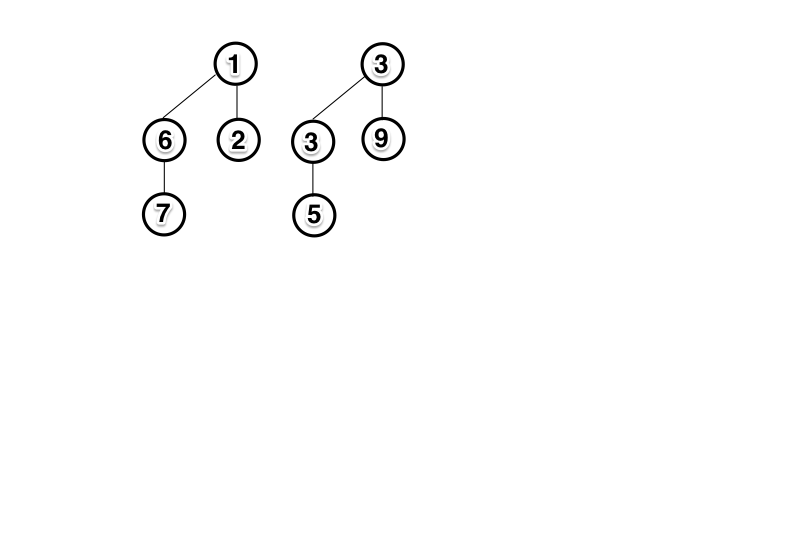
\includegraphics[height=5cm]{struct1.png}
      \end{figure}
    \end{column}
  \end{columns}

\end{frame}

% Exercise #3, cont ------------------------------------------------
\begin{frame}
\frametitle{Excercise: Binomial Heap Property \#2, Cont.}

  \begin{figure}
        \caption{Figure 4}
        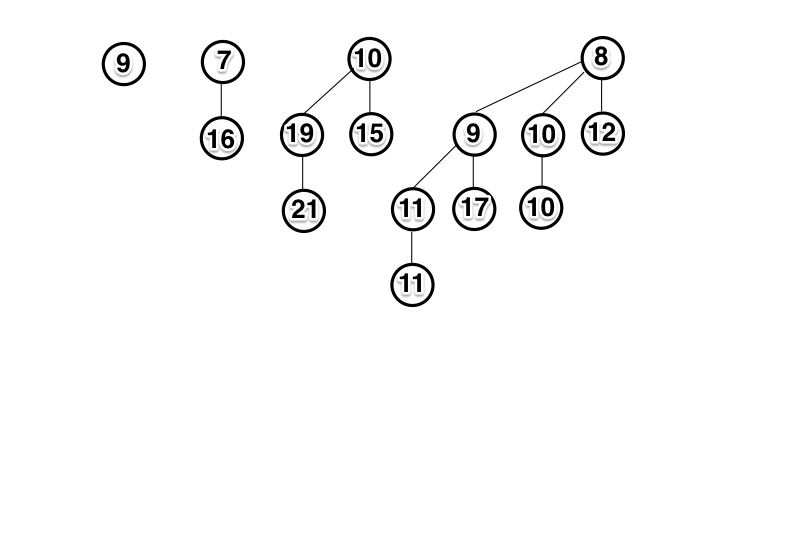
\includegraphics[height=7cm]{struct3.png}
      \end{figure}

\end{frame}
\end{document}